\documentclass{article}
\usepackage{graphicx} % if you need to include graphics
\usepackage{amsmath}  % if you need advanced math formatting
\usepackage{tikz}
\usepackage[a4paper, margin=3cm]{geometry}

\begin{document}
\section{Analysis}

\begin{center}
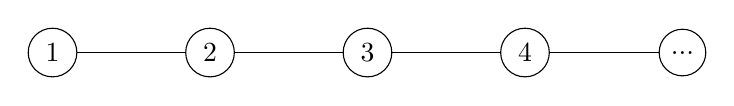
\begin{tikzpicture}
    \node (a) at (0,0) [circle,draw] {1};
    \node (b) at (2,0) [circle,draw] {2};
    \node (c) at (4,0) [circle,draw] {3};
    \node (d) at (6,0) [circle,draw] {4};
    \node (e) at (8,0) [circle,draw] {...};
    
    \draw (a) -- (b);
    \draw (b) -- (c);
    \draw (c) -- (d);
    \draw (d) -- (e);
\end{tikzpicture}
\end{center}
Let the network have a path graph (1-lattice graph) where subpopulation 1 is at the start of the path and has an initial infection of $I_1(0)=I_0$. The governing dynamics of the infection in subpopulation 1 is:

\begin{equation}
\dot I_1(t)=(\beta S_1-\gamma)I_1+\mu I_2-2\mu I_1
\end{equation}
Since $I_2$ starts at zero and the susceptible fraction starts at one, a first-order approximation can be made:
\begin{equation}
\dot I_1 \approx (\beta-\gamma-2\mu)I_1
\end{equation}
For a randomly selected subpopulation $j$, the infection fraction dynamics can be represented and approximated as:
\begin{equation}
\dot I_j =(\beta S_j-\gamma)I_j+\mu (I_{j-1}+I_{j+1}-2\mu I_j)
\end{equation}
Since the diffusion of infected individuals starts from index 1 and increasing, $I_{j+1} \approx 0$ with respect to $I_j$. Similar to the above linearization:
\begin{equation}
\dot I_j \approx \kappa I_j+\mu I_{j-1}
\end{equation}
where $\kappa = \beta-\gamma-2\mu$. Solving the differential equation for the linearized $\dot I_1$:
\begin{equation}
I_1 = I_0 e^{\kappa t}
\end{equation}
Substituting for $j=2$ in the equation above:
\begin{equation}
\dot I_2=\kappa I_j +\mu I_0 e^{\kappa t}
\end{equation}
This ODE can be solved analytically which results in:
\begin{equation}
I_2=I_0 \mu t e^{\kappa t}  
\end{equation}
Consequently, for $\dot I_3$:
\begin{equation}
\dot I_3=\kappa I_j +\mu^2 \kappa t e^{\kappa t}
\end{equation}
\begin{equation}
I_3 = I_0 \frac{\mu^2 t^2}{2} e^{\kappa t}
\end{equation}
Through induction, it can be found that:
\begin{equation}
I_j=I_0 \frac{\mu^{j-1} t^{j-1}}{(j-1)!} e^{\kappa t}
\end{equation}

To find the spread rate of the infection across the network, we solve for the time $t_{I_{j+1}=I_0} :=t_j$:
\begin{equation}
I_0 \frac{\mu^{j} t_j^{j}}{j!} e^{\kappa t_j} = I_0
\end{equation}
\begin{equation}
\frac{\mu^{j} t_j^{j}}{j!} e^{\kappa t_j} = 1 
\end{equation}
This unfortunately does not have a closed-form solution. However, a unique solution is guaranteed to exist, and since the function is monotonic and the root is simple, the solution can be found very easily numerically. To alleviate the numerical instability of higher and higher powers and factorial values, the log transform of the equation is solved instead:
\begin{equation}
\kappa t_j + j \ln(\mu t_j) - \ln(j!) = 0
\end{equation}

where the log of the factorial has very stable methods to solve\cite{C}.

To test this solution, the expected time for $I_j = I_0$ was found numerically through simulation of the ODEs for a path graph network and also computed numerically from equation (7).

\begin{figure}[!ht]
    \centering
    \includegraphics[width=120mm]{Figures/Pasted image 20240923204231.png}
    \caption{\small Simulation vs. analytical results for infection spread day. It can be seen that the time between $I_x(t)=i_0$ and $I_x(t)=sup(I_x(t))$ converges to a constant delay. Though this relationship, the spread infection days can be used to find the peak infection days.}
\end{figure}

It was found that equation (6) was remarkably accurate in estimating the spread infection day of the subpopulations. Furthermore, the peak infection day can be inferred from the spread infection day as they each converge to the same slope, and the offset between them is approximately the time taken for one subpopulation to reach the peak infection day starting from $I_0$.

Since we are interested in the spread rate of the infection, the objective is to derive the value ${\Delta t}_{j+1} := t_{j+1}-t_j$. To do so, we first use equation (7) to find $t_{j+1}$:

\begin{equation}
\kappa t_{j+1} + (j+1) \ln(\mu t_{j+1}) - \ln((j+1)!) = 0 
\end{equation}

Based on numerical results, we found that ${\Delta t}_{j}$ converges quickly to a constant value. Therefore, we apply an ansatz ${\Delta t}_{j+1} = t_{j+1} - t_j \approx {\Delta t}$ for $j \gg 1$, leading to $t_j \approx j \, \Delta t$.

Subtracting equation (7) from equation (8), we get:

\begin{equation}
\kappa \Delta t + j \ln\left( \frac{t_{j+1}}{t_j} \right) + \ln\left( \frac{\mu t_{j+1}}{j+1} \right) = 0
\end{equation}

After substituting $t_j \approx j \, \Delta t$, we find:

\begin{equation}
\kappa \Delta t + j \ln\left( \frac{j+1}{j} \right) + \ln\left( \mu \Delta t \right) = 0 
\end{equation}

Taking $\lim_{j \to \infty}$, and using $\ln\left( \frac{{j+1}}{j} \right) \approx \frac{1}{j}$, we get:

\begin{equation}
\kappa \Delta t + \ln( \mu \Delta t ) + 1 = 0
\end{equation}

This is still a transcendental function. However, a known solution for this equation uses the Lambert W function. Applying it here results in:

\begin{equation}
\Delta t = \frac{1}{\kappa} W\left(\frac{\kappa}{e \mu}\right)
\end{equation}

The next step is to derive the impact of the reactivity constant $\lambda$ on the spread rate and extrapolate this spread rate on more complex network topologies such as small-world networks and scale-free networks.

We again evaluate the same system but with individual restriction adaptivity, where $\bar \rho := 1 - \rho$ and $\rho(0) = 0$:

\begin{equation}
\dot \rho_{x,x'} = \lambda \mu \bar \rho (I_{x'} - I_x)
\end{equation}
\begin{equation}
\dot I_x = \beta S I - \gamma I +  \sum_{x'} \mu (I_{x'} - I_x) \bar \rho_{x,x'}
\end{equation}

We also define the flow $f_{x,x'}(t)$, which is the rate of incoming infected individuals per unit time from subpopulation $x$ into $x'$, where 

\begin{equation}
f_{x,x'}(t) = \mu \bar \rho_{x,x'} I_{x'}
\end{equation}

Applying the same linearization as equation (4):

\begin{equation}
\dot I_j \approx \kappa I_j + \mu \bar \rho I_{j-1} 
\end{equation}

Substituting $I_1 = i_0 \kappa e^{\kappa t}$ in equation (13):

\begin{equation}
\dot{\bar{\rho}}_2(t) = - i_{0} \lambda \mu \bar \rho_{2}(t) e^{\kappa t}
\end{equation}

The ODE in equation (13) can be solved using separation of variables as follows:

\begin{equation}
\dot{\bar{\rho}}_2(t) = - i_{0} \lambda \mu \bar \rho_{2}(t) e^{\kappa t}
\end{equation}

With the initial condition $\bar \rho_{2}(0) = 1$, we proceed as follows:
Dividing both sides by $\bar \rho_{2}$ and multiplying by $dt$, then integrating both sides:

\begin{equation}
\int \frac{1}{\bar \rho_{2}} \, d\bar \rho_{2} = - i_{0} \lambda \mu \int e^{\kappa t} \, dt
\end{equation}

\begin{equation}
\ln \bar \rho_{2}(t) = - \frac{i_{0} \lambda \mu}{\kappa} e^{\kappa t} + C_1
\end{equation}

Exponentiating both sides:

\begin{equation}
\bar \rho_{2}(t) = e^{C_1} e^{-\frac{i_{0} \lambda \mu}{\kappa} e^{\kappa t}}.
\end{equation}

Using $\bar \rho_{2}(0) = 1$ to find $C_1$:

\begin{equation}
\bar \rho_{2}(t) = e^{\frac{i_{0} \lambda \mu}{\kappa}} e^{-\frac{i_{0} \lambda \mu}{\kappa} e^{\kappa t}}
 = \exp\left(\frac{i_{0} \lambda \mu}{\kappa} \left( 1 - e^{\kappa t} \right)\right) 
\end{equation}

where $c := i_{0} \lambda \mu / \kappa$ is a dimensionless constant.

This shows that the rate of decay for the first applied restriction based on this adaptive strategy is super-exponential. This is an intuitive outcome of having the rate of change of $\rho$ be proportional to the incoming infected, which itself grows exponentially due to the internal infection rate. When simulating this system with sufficiently large $\lambda$, a somewhat unexpected result appears: it is found that adaptivity only delays the global infection spread instead of slowing down the spread rate. This can be seen in the infected evolution in all nodes in a simple SI epidemic model.

\begin{figure}[!ht]
    \centering
    \includegraphics[width=120mm]{Figures/Pasted image 20241026164447.png}
    \caption{\small Evolution of infected population in an adaptive SI model on a 1-lattice graph 
    (path graph) with $\lambda = 1e10$ and $i_0 = 1e-5$. It can be seen that there is a significant 
    delay between the infection in the first subpopulation (the one with an initial infected prevalence $i_0$, and the rest of the metapopulation. The spread rate among the rest of the network is the same as with no adaptivity.}
\end{figure}

\begin{figure}[!ht]
    \centering
    \includegraphics[width=120mm]{Figures/Pasted image 20241026170947.png}
    \caption{\small The same plot of the infected evolution in log-y scale. 
    Zero-values of infection have been omitted from this plot, all of which exist at day 1. 
    This scale helps show that the first subpopulation starts at an initial infected prevalence of 
    $i_0=1e-5$ and the grows exponentially, which can be seen by the constant-slope line of the evolution with a slope $1/\kappa$. This same exponential evolution can also be seen for subpopulation 2, quickly reaches the value of $F_2$ when $\rho_{2,1}$ reaches 1. A later figure will show the growth towards this value. Interestingly, the remainder of the subpopulations have a non-linear slope until it reaches the same threshold $F_2$ at which point their respective restriction completely shut down and their behavior turns purely exponential}
\end{figure}

\begin{figure}[!ht]
    \centering
    \includegraphics[width=120mm]{Figures/Pasted image 20241026192049.png}
    \caption{\small Evolution of mobility restrictions. It is worthy of note here that most $\rho$ values reach 1 significantly before the populaiton's corresponsponding infected prevalence reaches any significant value. It can be also seen from this plot that $\rho_2$ reaches 1 before the second day of the scenario, while $rho_3$ has a non-zero initial growth rate.}
\end{figure}

It is also worth noting that due to this super-exponential growth, $\rho_{2,1}$ decays down to zero much faster than the internal infection spread $I_2$. This difference in rates can be used to analytically approximate the delay in infection spread $t_2$ in subpopulation 2 from subpopulation 1. This can be done by first finding the final cumulative amount of incoming infecteds $F_2$ where 
$$F_2:=\int_0^\infty f_2(t)dt$$
where 

$$f_2(t)=\mu \bar \rho_2(t) I_1(t) = \mu \exp\left({c \left( 1 - e^{\kappa t} \right)}\right)i_0 e^{\kappa t} = \mu i_0 \exp\left({c \left( 1 - e^{\kappa t} \right)} +\kappa t\right)$$

An analytic solution for $F$ could be found using the exponential integral $\mathrm{Ei}$ function  $\int\exp(\exp(x))\,d x=\int{\frac{\exp(u)}{u}}\,d u={\mathrm{Ei}}(u)={\mathrm{Ei}}(\exp(x))$. However, a linearization of the exponent term was found to be sufficiently accurate based on the numerical simulation. We define the expression $E(t):=c\left( 1 - e^{\kappa t} \right)+\kappa t$ and linearize it around $t=0$: 
$$E(t)\approx (-c\kappa+\kappa)t = \kappa (1-c) t$$
substituting the linearized $E(t)$ and $f_2(t)$ back into $F_2$, we get:
$$F_2=\int_0^\infty \mu i_0 \exp\left(\kappa (1-c) t \right) dt = \frac{\mu i_0}{\kappa(c-1)}$$
dividing the numerator and denominator by $c=\frac{i_{0} \lambda \mu}{\kappa}$:
\begin{equation}
F_2=\frac{\frac{\kappa}{\lambda}}{\kappa\left( 1-\frac{1}{c} \right)}=\frac{1}{\lambda\left( 1-\frac{1}{c} \right)}
\end{equation}

While $F_2$ is evaluated from $t=0$ to $\infty$, due to the super-exponential rate of $f_2$, $F_2=F_2(\infty)\approx F_2(t_{f2})$ where $t_{f2}$ is a point in time where $\bar\rho(t_{f2})\approx 0$  $I({t_{f2}})\approx F_2$. This approximation can be validated by checking the value of $I_2$ in the numerical solution of the ODE at the point in time where $\bar\rho(t)\approx 0$ and check if $I(t)\approx F_2$. 

\begin{figure}[!ht]
    \centering
    \includegraphics[width=120mm]{Figures/Pasted image 20241027144236.png}
    \caption{\small Validation of $I_2$ approximation at $t \approx t_{f2}$. The $F_2$ Estimate is $1/\lambda$ which in a log-log scale has a slope of $-1$. As can be seen here, this approximation is only valid for $\lambda>1/i_0$. Before this threshold, there is approximately no dependency of $F_2$ on $\lambda$ }

\end{figure}

This observation allows us to solve a simplified version of the ODE $\dot I_2(t)$ starting from $t=t_f$, with the initial conditions at that point in time.
$$ I_2(t) = \int_{t_{f2}}^t \left(i_{0} \mu \bar \rho_{2}{(t)} e^{\kappa t} + \kappa I_{2}{\left(t \right)}\right) dt$$
since $\bar \rho \approx 0$ for $t\ge t_{f2}$ 
$$I_2(t) = \int_{t_{f2}}^t  \kappa I_{2}{\left(t \right)} dt = I_2(t_{f_2})e^{\kappa t} = F_2 e^{\kappa t} =\frac{e^{\kappa t}}{\lambda}$$
to find $t_2$, the value at which $I_2(t)=i_0$, 
$$I_2(t) =\frac{e^{\kappa t_2}}{\lambda}=i_0$$
solving for $t_2$:
$$t_2=\frac{\ln(i_0 \lambda)}{\kappa}$$
This relationship, as with the one for $F_2$, is only valid for $\lambda> \frac{1}{i_0}$. The most important observation from this finding is that the delay in infection depends on the logarithm of $\lambda$, which means there is very diminishing returns to increasing the adaptivity rates of travel restriction to infection. To validate this finding, $t_2$ was evaluated for different systems of ODEs with varying values of $\lambda$ and $\kappa$:

\begin{figure}[!ht]
    \centering
    \includegraphics[width=120mm]{Figures/Pasted image 20241027155933.png}
    \caption{\small Evaluation of $t_2$ for different $\lambda$ and $\kappa$ values with the $t_2$ approximation in a log-x scale. The straight line in this plot correponds to a logarithmic dependency of $t_2$ on $\lambda$, as was found in the analytical approximation. The approximation is only valid for $\lambda > i_0$, which is $10^5$ in this case. It can be seen that before this threshold, the impact of $\lambda$ is negligible and $t_2$ has the same value as if there was no adaptivity.}
\end{figure}

It can proven that, for a sufficiently large $\lambda$, $I_3(t_{F2})=\mu/\lambda$. (I just need to write it out and validate it numerically for different combination of $\mu$ and $\lambda$.

$$\dot I_2(t<t_{F2}) = f_2 = \mu i_0 e^{\kappa (1-c) t} \approx \mu i_0 e^{-\kappa c t}$$

$$I_2(t<t_{F2}) = \mu i_0 \left( \frac{e^{-\kappa c t}}{-\kappa c} - \frac{1}{-\kappa c} \right) = \frac{\mu i_0}{\kappa c}\left(1 - e^{-\kappa c t}\right) = \frac{1}{\lambda}\left(1-e^{-\kappa c t}\right) $$

$$\dot{\bar{\rho}}_3 = - \lambda \mu \bar{\rho}_3 \frac{1}{\lambda}\left(1 - e^{-\kappa c t}\right) =  - \mu \bar{\rho}_3\left(1 - e^{-\kappa c t}\right)$$

$$\int \frac{d{\bar \rho_3}}{\bar \rho_3} = \int \mu ( e^{-\kappa c t} -1)$$

$$\ln|\bar{\rho}_3| = \frac{- \mu e^{-\kappa c t}}{\kappa c} - \mu t + C_2$$

$$\bar \rho_3(t<t_{F2}) = \exp\left( \frac{1}{\lambda i_0} - \frac{e^{-\kappa c t}}{\lambda i_0}-\mu t\right) = \exp\left(\frac{1-e^{\kappa c t}}{\lambda i_0} - \mu t \right)$$

% $$\bar \rho_3(t<t_{F2}) \dot{=} \exp\left( \frac{1}{\lambda i_0} + \frac{{\kappa c t}}{\lambda i_0}-\mu t\right) = \frac{1}{\lambda i_0} + \mu t - \mu t = \frac{1}{\lambda i_0} $$

% $$f_3(t) = \mu \bar \rho_3(t)I_2(t) = \mu \exp\left( \frac{1}{\lambda i_0} - \frac{e^{-\kappa c t}}{\lambda i_0}-\mu t\right) \frac{1}{\lambda}\left(1-e^{-\kappa c t}\right)$$

% $$f_3(t) = \frac{\mu}{\lambda} \left( \exp\left( \frac{1}{\lambda i_0} - \frac{e^{-\kappa c t}}{\lambda i_0}-\mu t\right) - \exp\left( \frac{1}{\lambda i_0} - \frac{e^{-\kappa c t}}{\lambda i_0}-\mu t - \kappa c t\right) \right)$$

% $$f_3(t) \dot{=} \frac{\mu}{\lambda} \left( \exp\left( - \frac{{-\kappa c t}}{\lambda i_0}-\mu t\right) - \exp\left(  - \frac{{-\kappa c t}}{\lambda i_0}-\mu t - \kappa c t\right) \right) 
% = \frac{\mu}{\lambda}\left( 1 - \exp\left(- \kappa c t\right)\right)$$


%% ALTERNATIVE
Since $\lambda i_0 >>0$, the expression $\frac{1-e^{\kappa c t}}{\lambda i_0} \approx 0$. Hence, $$\bar \rho_3(t<t_{F2}) \approx e^{-\mu t}$$.

Substituting $\bar \rho_3$ into $f_3(t)=\mu \bar \rho_3(t) I_3(t)$, we get:
$$f_3(t)=\mu e^{-\mu t} \frac{1}{\lambda} \left(1-e^{-\kappa c t}\right) = \frac{\mu}{\lambda} e^{-\mu t}  \left(1-e^{-\mu \lambda i_0 t}\right)$$
Finding the indefinite integral of $f_3(t)$ $F_3(T) = \int_0^T f_3(t) dt$ (see appendix for integration)
\[
F_3(t) = \frac{1}{\lambda} \left( 1 - e^{-\mu t} - \frac{1}{1 + \lambda i_0} \left( 1 - e^{-\mu(1 + \lambda i_0) t} \right) \right) \approx \frac{1}{\lambda} \left( 1 - e^{-\mu t} \right).
\]

to find $t_3$, the time at which $I_3(t_3) = i_0$, we first integrate  $\dot I_3(t)$ for $I_3(t)<1/lambda$ where most of the growth is from incoming flow and then again for $1/\lambda<I_3(t)<i_0$.

$$\dot I_3(t) = \kappa I_3(t) + f_3(t) = \kappa I_3(t) +\frac{\mu}{\lambda} e^{-\mu t}  \left(1-e^{-\mu \lambda i_0 t}\right)$$

This can be solved for $I_3(t)$ (see appendix)

\[
I_3(t) \approx \frac{\mu}{\lambda (\mu + \kappa)} \left( e^{\kappa t} - e^{-\mu t} \right).
\]

with which we can solve for $t_{F_3}$ where $I_3(t)=F_3(\infty) = 1/\lambda$
$$I_3(t_{F_3}) \approx \frac{\mu}{\lambda (\mu + \kappa)} \left( e^{\kappa t_{F_3}} - e^{-\mu t_{F_3}} \right) \stackrel{!}{=}  \frac{1}{\lambda}$$
$$e^{\kappa t_{F_3}} - e^{-\mu t_{F_3}} =\frac{\mu + \kappa}{\mu}$$

Since $\dot I_3(t) \approx \kappa I_3(t)$ for $t>t_{F_3}$, which has the same evolution as $I_2(t)$, then $t_3 = t_2 + t_{F_3}$. Hence 
$ \Delta t_3 = t_{F_3}$
While one cannot solve explicitly for $t$ in this equation, it is important to observe that this approximation of $t_{F_3}$ is not a function of $\lambda$, which means that one cannot decrease the spread rate of infection for the third and onwards downstream neighbors. This result was confirmed to be sufficiently accurate through numerical testing. It was found that the spread rates of the third neighbor and beyond quickly converged to the infection spread rate of the non-adaptive case. This can be seen in the analytic approximation for large values of $t_{F_3}$ where $e^{\kappa t_{F_3}} - e^{-\mu t_{F_3}}  \approx e^{\kappa t_{F_3}}$

$$\Delta t_3 = t_{F_3} \approx \frac{1}{\kappa} \ln(1+\frac{ \kappa}{\mu})$$

This expression for $\Delta t_3$ is very close to equation (19) in the nonadaptive system, since $W(x) \approx ln(1+x)$. It is numerically found that in the adaptive system, for sufficiently large $i$, $$\Delta t_i \approx \frac{1}{\kappa} W(\frac{\kappa}{\mu})$$ 
Which further cements the finding that adaptivity only introduces a delay in infection spread in the immediate neighborhood of the first infected subpopulation while the remaining metapopulation network suffers from approximately the same infection spread rate as the unadaptive system. 

\end{document}